\chapter{Definition of Environment and Tools}\label{environment_and_tools}
This chapter lays the foundation for all following chapters by introducing the
environment in which this Master's Thesis has been created. First the \ac{UML}
and its profiling mechanism is described, followed by a concrete
example in terms of \ac{SysML}.
Furthermore Henshin, a graph transformation tool used in this integration process, is
explained in detail. Finally the three target tools of integration are
presented:
\textit{SiDiff}, \textit{SiLift} and the \textit{Patch-Tool}.
\section{UML and UML Profiles}\label{environment_and_tools:umlprofiles}
In the early 1990's the rising paradigm of \ac{MDSD} demanded modeling languages
for all domains and use cases, in which software development came to practical
use. As in figure~\ref{mdsd_history} depicted, many modeling languages have been
developed in this era. One among them was the \ac{UML}, which has been developed
by \textit{Grady Booch}, \textit{Ivar Jacobson} and \textit{James Rumbaugh} at
Rational Software\cite{Wik13_1}. It differentiated itself from other modeling
languages in its generic ideas and its wide support for modeling domains. Its
special and important role has been lifted drastically in the year 1997, as the
\ac{OMG} adopted \ac{UML} as modeling language. They fine tuned
the language and presented their version to the \ac{ISO} afterwards. The
\ac{UML} has been accepted as standard and published as Version 1.3 in 2000,
which can easily be called one of the big milestones for \ac{UML} and even for
\ac{MDSD} in general. Before standarization the industry hesitated to choose one
of the many modeling languages for their own usage, because it takes time and
money to develop tools which can handle each modeling language with its own
semantics. The paradigm change from coding to modeling has been delayed until
the standarization of modeling languages like the \ac{UML}. The \ac{OMG}
developed new versions of \ac{UML} with new features ever since, the actual
stable version used in practical environments is \ac{UML} 2.4.1 and has been
released in August 2011\cite{OMGUMLSpecification}, which is also the version
used throughout this Master's Thesis. 
\begin{figure}[h!]
\begin{center}
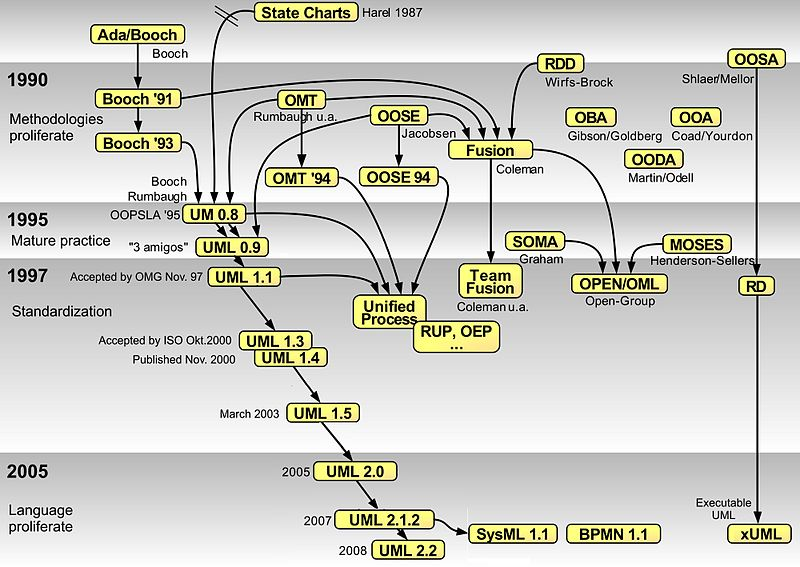
\includegraphics[scale=0.4]{mdsd_history}\\
\end{center}
\caption{Modeling languages history~\cite{Wik13_1}}
\label{mdsd_history}
\end{figure}

The \ac{UML} has been designed with many generic principles in
mind\cite{OMGUMLSpecification} such as:
\begin{itemize}
  \item Modularity
  \item Partitioning
  \item Extensibility  
\end{itemize}
Making use of these principles the \ac{UML} can be used to visualize practical
problems in many domains, using elements in combination like \textit{activies},
\textit{components} or \textit{use-cases}. An example of an \ac{UML} class
diagram, which is a very popular type of diagram in general, can be seen in
figure~\ref{uml_classdiagram}. This Master's Thesis emphasizes only on the
important parts of \ac{UML} for the integration, a more detailed and
comprehensive description of all possibilities the modeling language has to offer can be found in
\cite{UMLNutshell}.
\begin{figure}%[h!]
\begin{center}
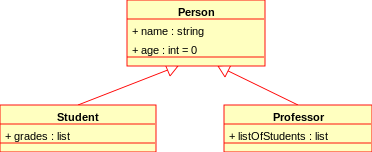
\includegraphics[scale=0.5]{uml_classdiagram}\\
\end{center}
\caption{\ac{UML} class diagram example~\cite{Wik13_2}}
\label{uml_classdiagram}
\end{figure}

Although the \ac{UML} supports a wide range of modeling domains, the principle
of \textit{extensibility} has been integrated deeply with its own mechanism: The
\ac{UML} profiling mechanism. The idea behind this mechanism is the possibility
for developers to define own modeling elements in \ac{UML} notation and
therefore add new semantics to an already known and widely supported modeling
language such as the \ac{UML}. Instead of defining a own modeling language for a
new given domain from scratch, a defined profile can alter a (sub)set of \ac{UML}
to provide a semantically more unterstandable way of modeling or additional
features, which have been missing in this particular area. An example of such an
profile definition is presented in figure~\ref{uml_profileexample}: Servers are
defined as profile for better understanding in this modeling domain. They extend
the \ac{UML} with its own semantics, such as the relationship between a
\textit{device} and a \textit{server}. 
\begin{figure}%[h!]
\begin{center}
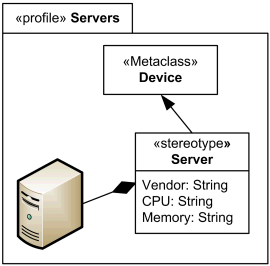
\includegraphics[scale=3.5]{uml_profiled}\\
\end{center}
\caption{Profile Application Example~\cite{UMLprofiled}}
\label{uml_profileexample}
\end{figure}

All \ac{UML} profiles are defined in an \textit{additive} manner. This basic
principle leads to conformity between unprofiled and profiled \ac{UML} models, therefore no new modeling tools are
needed if they already support all features of \ac{UML}. This is a tremendous
advantage over other modeling languages, which do not facilitate such
extensibility in this generic way or at all. Another example exposing this can
be imagened easily:
The technology of connected devices like tablets or new server backends like clouds are using a
new way of network connectivity. To cope with this new area of problems in a
\ac{MDSD} way there has to be a modeling language and modeling tools capable of
such modeling elements and their relationships. Using the \ac{UML} profiling
mechanism no new modeling tools are needed, all semantics of this new domain
are modelled within \ac{UML} profiles, such as relationships between cloud
servers and its clients.

These are just small examples of what possibilities are available via the
profiling mechanism. Other popular examples which are using this functionality extensively are \ac{MARTE} and \ac{SysML}, which will be explained in detail in the
following section.
\section{SysML}\label{environment_and_tools:sysml}
One example of making use of the \ac{UML} profiling mechanism is the \ac{SysML}
profile, which defines new semantics to existing elements in the \ac{UML} and
extents the modeling language with new elements and diagrams. The profile is
used in  and has been developed for the domain of systems engineering applications.
Like \ac{UML}, \ac{SysML} has been adopted by the \ac{OMG} and its specification
has first been published officially in September 2007\cite{Wik13_3}. The current
version in use is \ac{SysML} 1.3, which was issued by the \ac{OMG} in June 2012
\cite{OMGSysMLSpecification}.

\ac{SysML} tries to reduce the scope of modeling elements of \ac{UML} by using
only a subset of all elements available as depicted in figure
\ref{sysml_uml_relation}. The wide support of modeling domains and elements of
\ac{UML} can lead to confusion among developers, which \ac{SysML} tries to solve
by only using domain specific elements in the area of systems engineering.

\begin{figure}%[h!]
\begin{center}
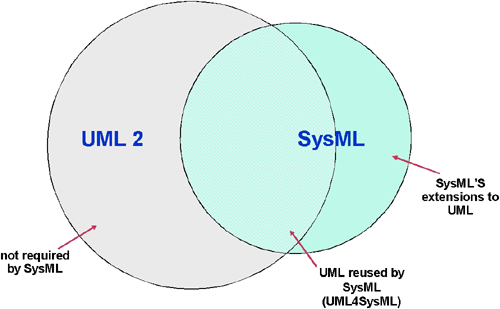
\includegraphics[scale=0.4]{sysml_uml_relation}\\
\end{center}
\caption{Relationship between \ac{UML} and \ac{SysML}~\cite{OMGSysML}}
\label{sysml_uml_relation}
\end{figure}

Additionally parts of \ac{UML} have been changed in semantics and new diagrams
have been introduced. A \ac{SysML} diagram overview is presented in figure
\ref{sysml_overview}.

\begin{figure}[h!]
\begin{center}
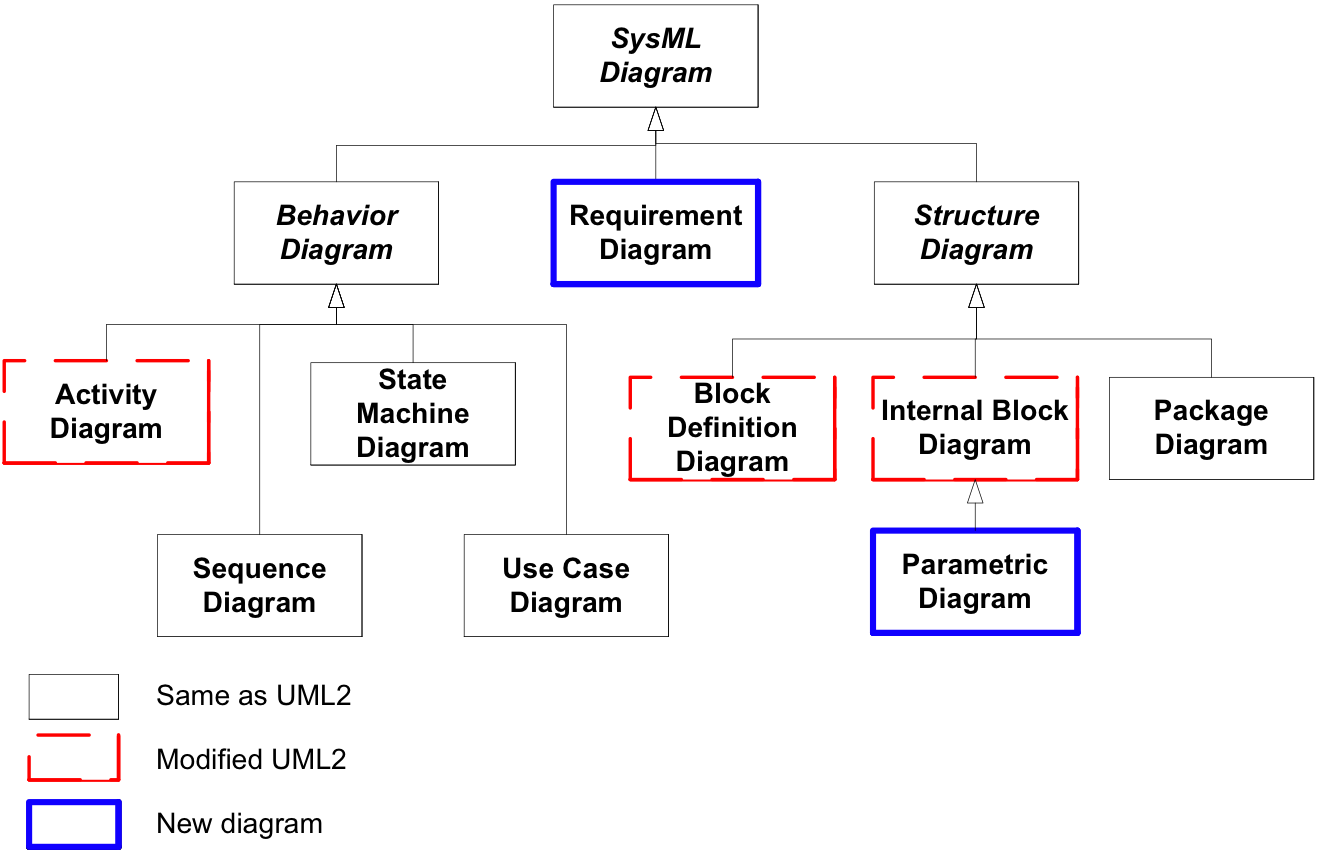
\includegraphics[scale=0.5]{sysml_overview}\\
\end{center}
\caption{The SysML diagram taxonomy~\cite{OMGSysMLSpecification}}
\label{sysml_overview}
\end{figure}

 The new diagrams introduced in \ac{SysML} shall be explained:
 
\textbf{Requirement Diagram}\\
Systems engineering is mostly driven requirement-based, therefore this new type
of diagram meets this design principle. In this domain a requirement can be
modeled graphically and contains properties and/or conditions which must be
satisfied. Requirements can have relationships between modeling elements, which
can also be requirements themselves. Another feature is the reuseability across
product families and projects, which is realized through the namespace
containment in \ac{SysML}.

\textbf{Parametric Diagram}\\
As seen in figure~\ref{sysml_overview}, the parametric diagram has a direct
relationship to the internal block diagram, which contains the basic modeling
elements of \ac{SysML}. The idea is to offer the possibility to describe
constraints among properties between these basic elements such as
\textit{Blocks}.
Behavior and structure models can be integrated easily with engineering analysis like
performance or reliability, which often occur in systems engineering domains.

Additionally many modififications have been implemented to conform to the
systems engineering common language and principles in software design, making
them more understandable for developers from this particular domain. A basic
example for this is the \ac{UML} \textit{Class} element extension by
the \ac{SysML} \textit{Block} element. This seems appropiate because of the common usage of mechanical or electrical parts, which do not conform to the semantic of \textit{Class}.
A more detailed overview and description of all elements, which are
introduced by \ac{SysML} and how they are used can be found in
\cite{OMGSysMLSpecification} and~\cite{SysMLEngineering}.
\section{Henshin}\label{environment_and_tools:henshin}
Contrary to text-based tools, modeling tools are based on graph
representations as input. A model can be defined as graph, consisting
of nodes representing the modeled element instances and edges representing
relationships between them. Henshin is built upon this foundation of model representation,
whereas the name Henshin originates from Japanese and translates to
\textit{transformation}.
It has been developed as a joint project by developers at the
Philipps-University in Marburg, the Hasso Plattner Institute in Potsdam, 
the Technical University of Berlin, and others~\cite{Henshin}. The first version
of Henshin, 0.8.0, has been released in September 2011, and Henshin has been in
development ever since. The current stable version is 0.9.8, which this Master's
Thesis uses throughout the whole integration process. 

Based on the theory of graph transformation\footnote{Often also
called graph rewriting}, Henshin provides the functionality of transformating a
given model based on defined Henshin rules. The tool itself is implemented for
the \ac{EMF} and can be used within this context. Like compilers in text-based
tools, graph-transformation tools are trying to find a match on the \ac{LHS} and transformate this match
based on a given rule into a result on the \ac{RHS}. In figure~\ref{graphrewriting_example} the \ac{LHS},
denoted as $L$ is transformed into the \ac{RHS} denoted as $R$. A
multiplication with $2$ is transformed into an addition of the digit with
itself. The corresponding match on the \ac{LHS} and result on the \ac{RHS} are
denoted in dashed lines. This rudimentary definition and example are sufficient
in this context, for a in-depth view on graph transformation and the theory
behind~\cite{rozenberg1997handbook} can be recommended.

\begin{figure}%[h!]
\begin{center}
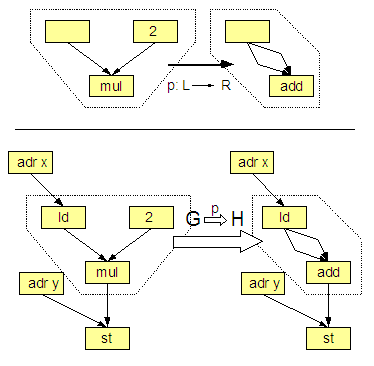
\includegraphics[scale=0.5]{GraphRewriteExample}\\
\end{center}
\caption{Graph transformation example~\cite{Wik13_4}}
\label{graphrewriting_example}
\end{figure}

For using Henshin the definition of Henshin rules is essential: Henshin rules
are used as input language for the transformation process, additionally to the
input model itself. Using the graphical Henshin diagram syntax, a defined rule
looks similar to the example rule in figure~\ref{Henshinrule_example_1}. There are
five types of nodes in a Henshin rule, whose semantics correspond to the five
type of edges:
\begin{itemize}
  \item \textbf{Create} \\
  	    A create node exists only in the \ac{RHS} of the input model and is
  	    therefore created in the result model.
  \item \textbf{Delete} \\
  	    A delete node exists only in the \ac{LHS} of the input model and is
  	    therefore deleted from the input model.
  \item \textbf{Preserve} \\
        A preserve node exists in both sides of the input model, \ac{LHS} and
        \ac{RHS} that is. These nodes are used as a match in \ac{LHS} and are not altered in the result model.
  \item \textbf{Forbid} \\
        A forbid node, or \ac{NAC}, defines which
        elements are not allowed to be matched in the \ac{LHS} for executing the
        transformation. If one forbid node is found in the input model, the
        transformation can not be executed.
  \item \textbf{Require} \\
        A require node, or \ac{PAC}, defines which
        elements must be matched in the \ac{LHS} for
        executing the transformation. If one require node is not found in the
        input model, the transformation can not be executed.
\end{itemize}
\begin{figure}[h!]
\begin{center}
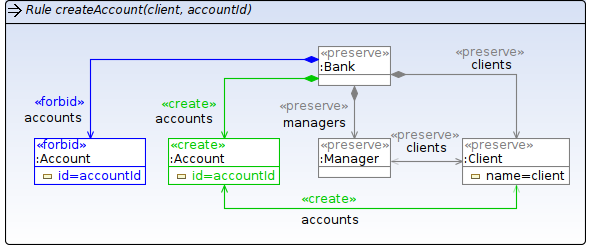
\includegraphics[scale=0.4]{rule-create-account}\\
\end{center}
\caption{Henshin rule example (1)~\cite{Henshin}}
\label{Henshinrule_example_1}
\end{figure}

Using these types of nodes and edges, describing relationships between
nodes, one can use Henshin for transformating a given input model.
The example shown in figure~\ref{Henshinrule_example_1} creates a bank account
for a client by transformating a given input model conforming to a meta model
describing a bank and its relationships to its accounts, managers and clients.
The forbid node on the left represents the constraint that no two accounts managed by the same bank may
have the same account id. The parameters which are given to the Henshin rule
should also be mentioned, they can be a primitive type like a \textit{String} or
a object parameter and are used for the execution. The transformation engine of
Henshin itself executes a Henshin rule as follows:
\begin{enumerate}
  \item Search for a match in input model, defined via preserve nodes and their
  relationship to other nodes.
  \item Check if no forbid node could be matched or a require node could not be
  matched.
  \item Create all create / delete all delete nodes and edges describing their
  relationship.
\end{enumerate}
A special feature of Henshin Rules are presented in figure
\ref{Henshinrule_example_2}: Nested rules. The delete node is marked with a
star operator and therefore will be executed as many times as possible. In this
particular example all accounts of a client will be deleted instead of only
one as if not defined as nested rule. Internally the Henshin interpreter will
try to match the preserve nodes and edges after each successfull execution and
if it succeeds, it will execute the transformation again. This feature is important
for later use and therefore is explicitly mentioned and explained.
\newpage
\begin{figure}[h!]
\begin{center}
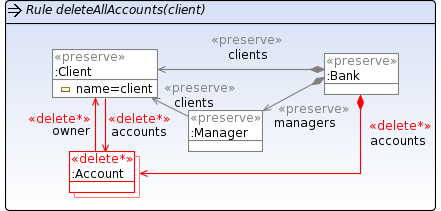
\includegraphics[scale=0.5]{rule-delete-all-accounts}\\
\end{center}
\caption{Henshin rule example (2)~\cite{Henshin}}
\label{Henshinrule_example_2}
\end{figure}

Using Henshin as a tool, it offers different ways of executing Henshin
rules for transformation. They can be executed either via the Henshin
graphical interface, or via the Henshin interpreter \ac{API}, which can be
called using programming languages like Java. All described tools in this
Master's Thesis are based on the latter option. Because Henshin offers more
features than described in this section, publications of the developers of
Henshin like~\cite{henshinpublication} are recommended as additional lecture.
\section{SiDiff}\label{environment_and_tools:sidiff}
As mentioned in the introduction do modeling tools need to support features
known from text-based tools. One important aspect for parallel development
paradigms is the detection of correspondences and differences between two
different revisions of software. In the area of \ac{MDSD} 
software consists of models, therefore such features must be available in this
context. The SiDiff tool environment~\cite{SiDiffURL} offers such
functionalities: It can derive correspondences and differences between two
models meta model-independent. The basic concept and tool implementation was
released in 2004 by the \ac{SEG}~\cite{SEGURL}, whereas this version can be
defined as proof of concept. The version in today's use was initiated in 2009,
it has been revamped from scratch and implements a new software architecture
built upon \textit{OSGi} and the Eclipse plugin ecosystem. SiDiff is built upon
a service-based architecture internally, which eases the integration of new
services in any part of the computing pipeline including the matching itself.
\newpage
\begin{figure}[h!]
\begin{center}
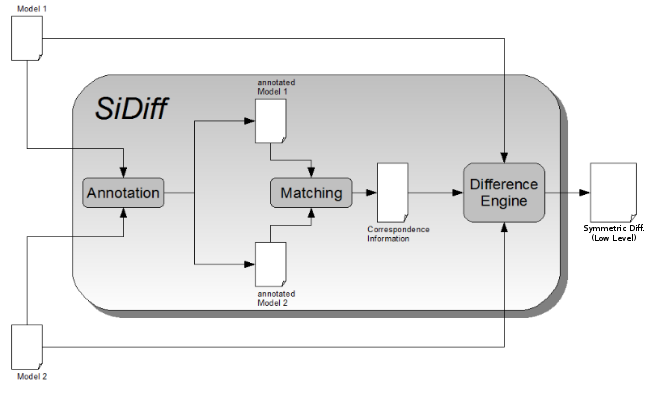
\includegraphics[scale=0.5]{sidiffworkflow}\\
\end{center}
\caption{SiDiff workflow~\cite{SiDiffURL}}
\label{sidiffworkflow}
\end{figure}

SiDiff make use of the computing pipeline depicted in figure
\ref{sidiffworkflow}: Two models are used as input for comparison and are
annotated for later processing of the implemented matching services. One big
advantage of SiDiff is its vast configuration possibility, which emphasizes
its generic approach. In this step of pipeline the configuration defines which
model elements are annotated and how this is done. The SiDiff matching services
are then computing correspondences on the resulting annotated
models, whereas the current available matching services consist of:
\begin{itemize}
  \item  \textbf{ID-based Matcher} \\
  		This matcher makes use of given \ac{UUID}s, if available. Elements of Model
  		$1$ are corresponding to Elements of Model $2$ if and only if their
  		respective \ac{UUID} is equal.
  \item  \textbf{Signature-based Matcher} \\
  	 	This matcher is based upon signatures of elements, which can be computed by
  	 	taking attribute values or relationships into consideration. Which
  	 	properties are used for the creation of signatures is defined via a
  	 	configuration file.
  \item  \textbf{Similarity-based Matcher} \\
  		This matcher computes a similarity between elements, and if they reach a
  		given threshold they are declared as corresponding. This part of SiDiff
  		can be configurated in enormous detail, for example which element attributes
  		are weighted in comparison to others. This matcher and its
  		configuration is to comprehensive to discuss in detail, a more
  		detailed look is given in~\cite{KellerWN05}.
\end{itemize}
The matching result defines which elements of Model $1$ are  corresponding to
which elements of Model $2$ only, therefore a difference engine is executed
afterwards for detecting unmatched elements. The final result is a 
symmetric difference, which consists of both the correspondences and the differences 
between the input models as seen in figure~\ref{symmetricdiff}. The differences
are presented on a low-level of abstraction.

\begin{figure}[h!]
\begin{center}
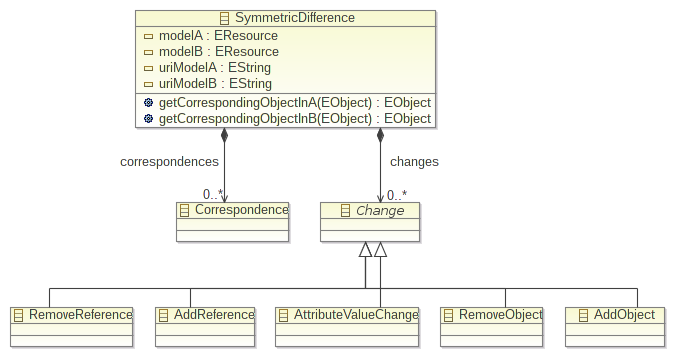
\includegraphics[scale=0.6]{SymmetricDiff}\\
\end{center}
\caption{Symmetric Difference (snippet)~\cite{SiDiffURL}}
\label{symmetricdiff}
\end{figure}

The computed symmetric difference lays the foundation for other
tools, which can now use the given information for their own advantage. One
tool, which can use the symmetric difference computed by SiDiff as input is
SiLift, which will be presented in the following section.
\section{SiLift}\label{environment_and_tools:silift}
A symmetric difference created generically presents its differences on a
low-level of changes, which can be hard to comprehend by developers as they may
differ significantly from the expected changes. SiLift, as the name suggests,
lifts this low-level changes onto a higher abstraction level consisting of edit
operations. SiLift itself is in development since 2011~\cite{rulebaseapproach}
by the \ac{SEG}~\cite{SEGURL} and is today implemented as proof-of-concept tool
embedded into the Eclipse plugin ecosystem~\cite{modelevolutionlifting}. As
SiDiff, Silift has taken an generic approach in the support of modeling language
and its software architecture.

 \begin{figure}[h!]
\begin{center}
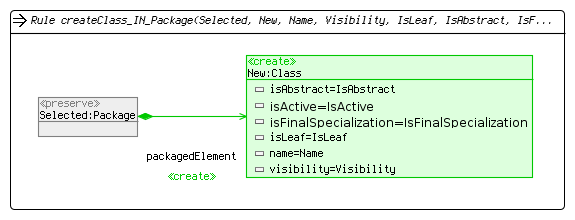
\includegraphics[scale=0.7]{CREATE_Class_IN_Package}\\
\end{center}
\caption{Edit operation defined via Henshin rule}
\label{create_class_in_package}
\end{figure}

The basic idea of the lifting process is to use Henshin rules as edit operation
definitions and detect changes using these rules. A small \ac{UML} example is
shown in figure~\ref{create_class_in_package}: The Henshin rule tries to match a
\textit{Package} and creates a \textit{Class} within the detected package. The
rule describes the edit operation of creating a class in a package. If this
Henshin rule is executed successfully it will create a class in a package,
corresponding to a edit operation executed by the developer. Such edit rules can
be generated via the \ac{SERGe}~\cite{SERGEURL} or manually created, as
depicted in the top of figure~\ref{siliftworkflow}. The execution of a edit rule
itself creating or changing the input model in the operation
detection is not desired. Therefore the edit rules are transformed
into recognition rules, which are Henshin rules themselves. They are responsible
for the detection of a possible execution of the originated edit rule.
There are two different types of edit rules:

\textbf{Atomic edit rules} \\
These rules are defined as \textit{atomic} as they are essential for detecting
all possible changes for this type of input model and can not be reduced to
smaller pieces. They are mostly generated by \ac{SERGe}.

\textbf{Complex edit rules} \\
These rules consist of $2$ or more atomic rules, defining an even higher level
of abstraction. They must be manually created, as they can not be deduced from
the meta model of the input models. The creation requires a very good knowledge
in the particular domain.
\newpage
 \begin{figure}[h!]
\begin{center}
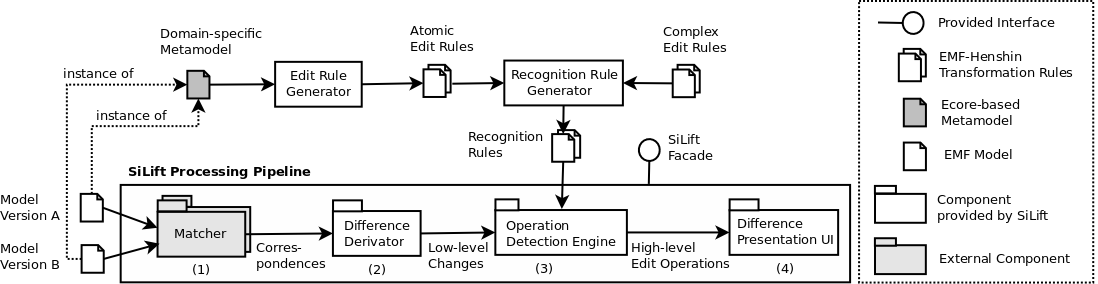
\includegraphics[scale=0.25]{siliftworkflow}\\
\end{center}
\caption{SiLift work flow~\cite{SiLiftURL}}
\label{siliftworkflow}
\end{figure}

As illustrated in figure~\ref{siliftworkflow}, the SiLift processing pipeline
consists of different stages:
\begin{enumerate}
  \item  \textbf{Matcher} \\
  		This matcher can be exchanged by any matching service, for example EMF
  		Compare or the more sophisticated SiDiff matcher explained in the preceding
  		section.
  \item  \textbf{Difference Derivator} \\
  	    In this step the low-level changes are derived from the symmetric
  	    difference provided by the matcher.
  \item  \textbf{Operation Detection Engine} \\
  		This part of the processing pipeline can be called the \textit{core} of
  		SiLift, as it implements the lifting of the low-level changes onto a edit
  		operations level of abstraction. It uses recognition rules as input for the
  		detection of these edit operations.
  \item  \textbf{Difference Presentation UI} \\
  		Another shortcoming of low-level changes is the presentation of the
  		mentioned. SiLift presents the now lifted changes visually to the user,
  		for a more comprehensive understanding of the detected changes.
\end{enumerate}
The final result of the whole SiLift processing pipeline is a lifted symmetric
difference, which contains edit operations as changes. These changes can be
interpreted as an directed asymmetric difference between two input models.  
Such an edit operation script, which is often called a \textit{Patch}, can be
used to perform these changes made between these models on another input model.
The following section describes such a tool for the creation and application of
a patch, consisting of edit rules as list of changes.
\section{Patch-Tool}\label{environment_and_tools:patchtool}
Considering that a symmetric difference has been created and lifted beforehand,
the Patch-Tool now uses a asymmetric difference, which can be deducted from a
symmetric difference, as input for creating and applying such a list of
operations. The Patch-Tool has been developed by the \ac{SEG}~\cite{SEGURL} in
2013, and is based upon the results from SiDiff and SiLift. As the other tools,
the Patch-tool is also implemented in the Eclipse ecosystem and its architecture
implements interfaces, enabling the exchange of the matcher beforehand
or even the transformation engine. 

 \begin{figure}[h!]
\begin{center}
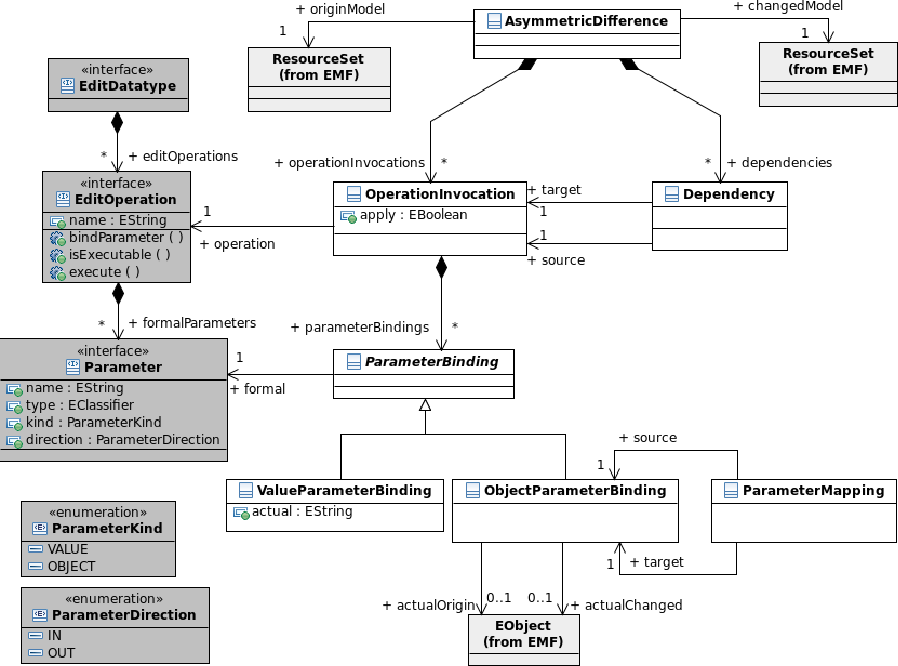
\includegraphics[scale=0.4]{patchoverview}\\
\end{center}
\caption{Patch overview~\cite{kochpatchen}}
\label{patchoverview}
\end{figure}

As mentioned in section~\ref{environment_and_tools:silift} is the execution of
a Henshin rule corresponding to a edit operation executed by the developer. The
Patch-Tool now orders the edit operations, also called \ac{SCS}, considering
dependencies between them as seen in
figure~\ref{patchoverview}~\cite{modelevolutionlifting}. One dependency
can be used for demonstration purposes: \textit{Create-Use}. If one wants to
change the name of a \textit{Class}, the class has to be existing previously.
The operation for creating the class and setting its name therefore have got such
a dependency between them. A more detailed look at dependencies, whether it be
their declaration or their detection can be glimpsed
at in~\cite{modelevolutionlifting}.

As depicted in figure~\ref{patchoverview} will the Patch-Tool create the
binding of parameters by finding corresponding ones in the target model.
The final result is a ordered list of \textit{OperationInvocations}, which have
been constructed with corresponding parameters. After the creation of such a
patch it is then applied to the target model, which will transform the model
according to the patch using the defined transformation engine, Henshin in this
case.
